\subsection{Kiến trúc hệ thống}
\begin{figure}[H]
    \centering
    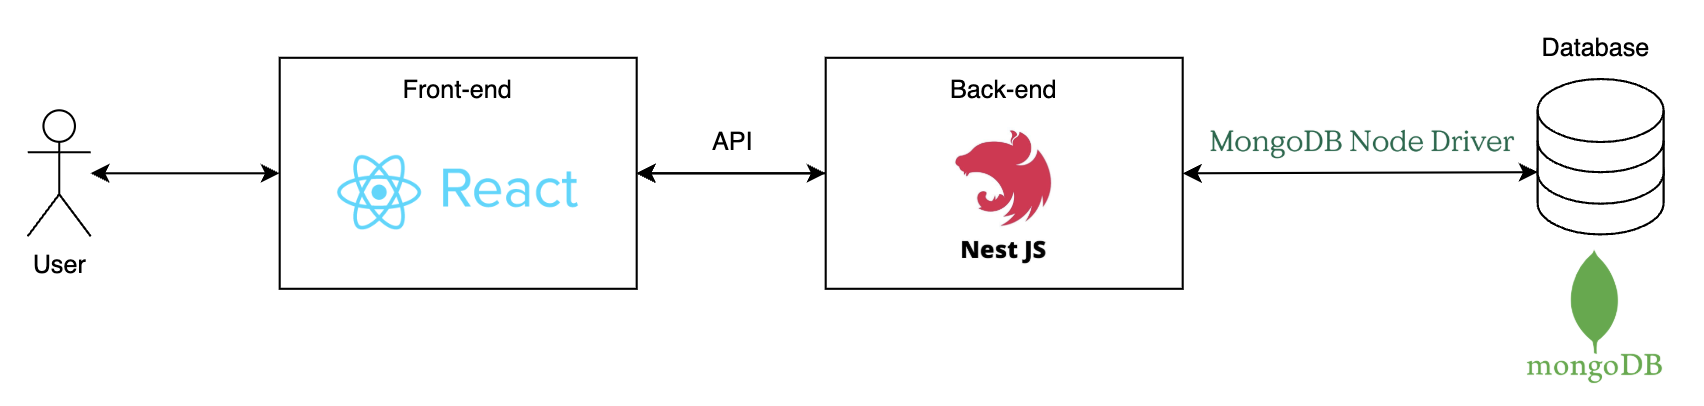
\includegraphics[width=\linewidth]{DBMS-Application/Images/dbms-architecture.png}
    \caption{Kiến trúc hệ thống}
\end{figure}

Kiến trúc của hệ thống là \textbf{Client-Server Architecture}, cụ thể là \textbf{3-Tier Architecture} (kiến trúc 3 lớp), gồm các tầng sau:
\begin{itemize}
    \item \textbf{Tầng Presentation (Client)}:
    \begin{itemize}
        \item Thành phần: \textbf{React.JS (Front-end)}
        \item Vai trò: Hiển thị giao diện người dùng, xử lý các thao tác và yêu cầu từ phía người dùng. Tầng này gọi API từ Back-end và hiển thị dữ liệu trả về.
    \end{itemize}

    \item \textbf{Tầng Application Logic (Server)}:
    \begin{itemize}
        \item Thành phần: \textbf{Nest.JS (Back-end)}
        \item Vai trò: Xử lý logic nghiệp vụ, xác thực người dùng, điều hướng các yêu cầu đến cơ sở dữ liệu, và trả kết quả về cho Front-end thông qua API.
        \item Kết nối tới cơ sở dữ liệu sử dụng \textbf{MongoDB Node Driver}.
    \end{itemize}

    \item \textbf{Tầng Data (Database)}:
    \begin{itemize}
        \item Thành phần: \textbf{MongoDB}
        \item Vai trò: Lưu trữ và quản lý dữ liệu của hệ thống, xử lý các thao tác truy vấn, thêm, sửa, xóa dữ liệu.
    \end{itemize}
\end{itemize}

\textbf{Quy trình hoạt động}:

\begin{figure}[H]
    \centering
    \begin{tikzpicture}[node distance=1.5cm]
    % Các khối trong quy trình
    \node (user) [startstop] {1. Người dùng tương tác với giao diện (Xem danh sách công việc, ứng tuyển công việc,...)};
    \node (frontend) [process, below of=user] {2. Front-end gửi request đến Back-end qua API};
    \node (api) [process, below of=frontend] {3. Back-end xử lý logic nghiệp vụ và truy vấn CSDL MongoDB};
    \node (response) [process, below of=api] {4. Back-end gửi phản hồi về Front-end};
    \node (display) [startstop, below of=response] {5. Front-end hiển thị dữ liệu lên giao diện người dùng};
    
    % Vẽ các mũi tên
    \draw [arrow] (user) -- (frontend);
    \draw [arrow] (frontend) -- (api);
    \draw [arrow] (api) -- (response);
    \draw [arrow] (response) -- (display);
    
    \end{tikzpicture}
\end{figure}